%=========================================================================
% (c) Michal Bidlo, Bohuslav Křena, 2008

\chapter{Introduction}
Virtualization has become very important and powerful tool used in various technology sectors. There are plenty of usecases including testing, learning and development. Availability and improvement of open source technologies is making this area even more competitive. As datacenters grow, there are several aspects that need to be considered, when choosing the most suitable solution.

oVirt\cite{oVirt} provides complete stack of management functions allowing to control and monitor the whole realm of virtual datacenters. The presence of rich Restful API, even allows us to build our own custom tools such as moVirt\cite{moVirt} and Ansible\cite{Ansible}. 

Nowadays, the internet is being overwhelmed by modern single page applications created by advanced Javascript frameworks. This paper is written around the project, which makes effort to build similar application for oVirt. Main focus will be placed on dialogs as they administrate big entities like virtual machines and templates. Each of those entities has huge number of fields that might be in relation with one another. The challenge is to make dialogs quick, responsive and force them to always provide valid data. Regarding data validity there are two specials cases. The first case represents fact, that many of fields can be prefigured from template. The other one is a case when we need to edit particular entity, so it is crucial to display data belonging to right entity, which needs to be edited. This points to the fact, that dependency handling and excellent state management based on decision made by user can influence the data in one or few other fields.

Redux is technology designed especially for state management of React\cite{React} applications. There are some recommendations not to use Redux\cite{Redux} to manage state of dialogs. Configuration dialogs of oVirt entities can contain up to 62 fields \ref{graph}. Verifying data throughout whole configuration process, field after field, via technologies like jQuery can lead to pretty complex code. This is the reason why thoroughly designed solution for state management is required. But in this case, it is so complex that it is necessary to know the values in various fields to make sure that user is selecting valid data. Template belonging only to certain cluster provides good example.

React allows us to create presentional part of application. Similiarly like Redux, React itself has mechanisms to manage state of components, but as our application expands, large number of components may cause problems which lead to birth of Redux. This project is developed with open source spirit and so is the project design delivered by Patternfly\cite{Patternfly} library of elements.


\chapter{oVirt}
oVirt is an open source virtualization management tool that provides centralized management of virtual datacenters, virtual hosts, virtual machines, storage and networking infrastructure. oVirt platform consists of two main parts - an oVirt engine and one or more oVirt nodes.

\section{oVirt engine}
oVirt engine represents the part where all management features resides. Backend is written in Java, from frontend perspective it offers multiple ways to manage virtual datacenters.

\begin{figure}[h]
\center{\scalebox{1}{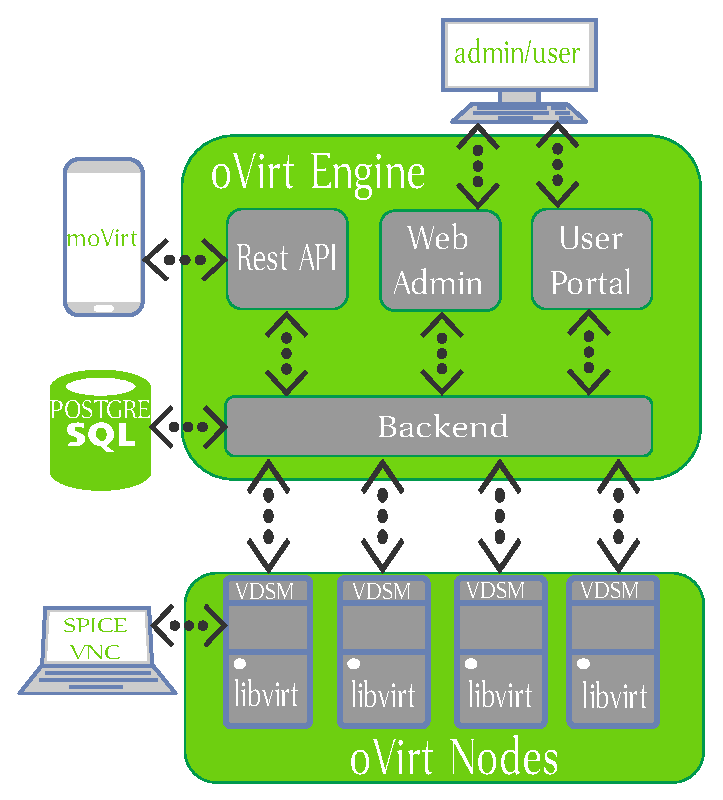
\includegraphics{architecture.eps}}}
\caption{oVirt architecture \cite{oVirtImg}}
\label{vector}
\end{figure}

\subsection{Administration portal}
Administration portal is web based tool able to manage all available resources with user management, permissions and monitoring. 

\subsection{User Portal}
More suited for end users is User Portal as it targets basic virtual machine management and access to virtual consoles secured by protocols SPICE\cite{SPICE} and VNC\cite{VNC}. User has only access to virtual machines and resources which was allocated to him by administrator.

\subsection{Rest API}
External applications may influence datacenter management thanks to RESTful API. As a demonstration can be used Android application moVirt, which allows to manage and monitor datacenter from a smartphone. oVirt Rest API supports both XML and JSON formats and it will be crucial part of development part described in this document.

\section{oVirt node}
Resources managed by oVirt engine belongs to one or more oVirt nodes, which are basically servers running RHEL, Fedora on Centos with enabled KVM hypervisor and VDSM(Virtual Desktop and Server Manager) daemon. VDSM deamon has control of all available resources including storage, networking and virtual machines. It is also responsible for reporting all actions to engine.

\section{oVirt Entities}
Data managed by oVirt are structured to objects known as entities. Next few sections are focused on explanation of oVirt entities important for this thesis.

\textbf{Cluster} is logical group of virtual machines sharing the same storage domain and have the same CPU architecture of CPU family.

\textbf{Template} represents a copy of virtual machine. This functionality is very valuable especially in cases when you need to repeatedly create bigger amount of virtual machines with same of similar properties. Template also holds the information about hardware and software configurations of derived virtual machine. Once a virtual machine based on certain template is created, template cannot be removed while the virtual machine exists in the environment. 

\textbf{Virtual Machine} can be explain as actual computer system running in emulated environment and providing as much functionality as actual physical compute would provide.

\textbf{Host} is physical computer with installed hypervisor which allows to run multiple virtual machines on this host. oVirt usually has multiple host machines that are able to run as many virtual machines as resources low.

\chapter{Manage IQ}
ManageIQ\cite{ManageIQarchitecture} is open source cloud management tool able to manage environments of different sizes. With support for platforms like oVirt, Open Stack, Kubernetes, Amazon Web Services, Google Cloud Platform, Microsoft Azure and many more allows user to control multiple technologies such as virtual machines, public clouds and containers from multiple vendors in one modern web application.
Application itself is written in Ruby and it can be deployed as virtual machine image and Docker container.

\begin{figure}[h]
\center{\scalebox{0.75}{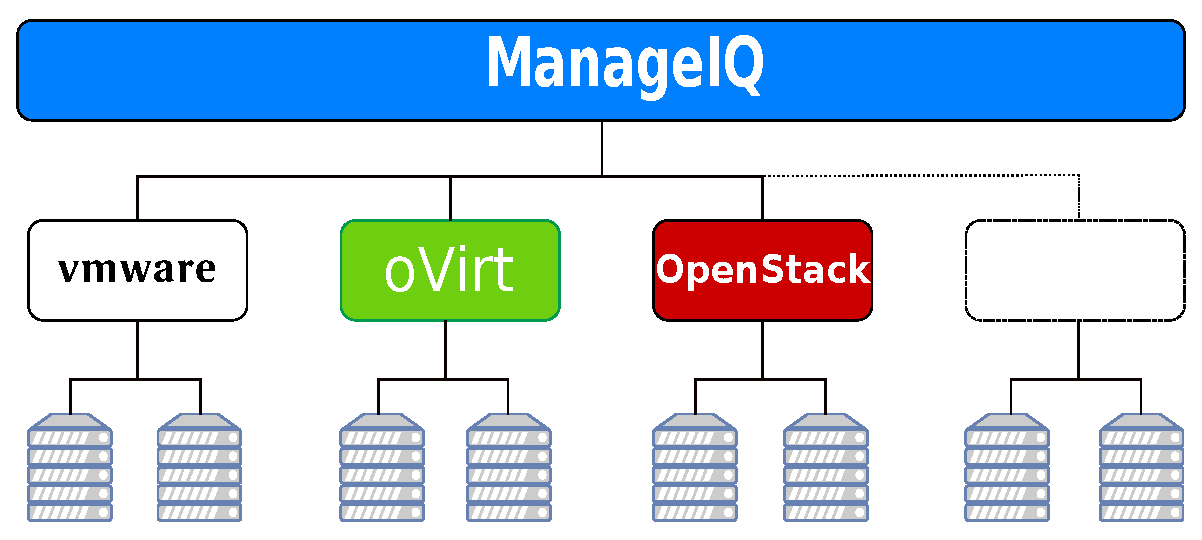
\includegraphics{manageIQ.eps}}}
\caption{ManageIQ overview}
\label{vector}
\end{figure}
\section{Discovery}
All platforms supported by ManageIQ are providing APIs. By integrating these API functions, ManageIQ can scan the environment and discover all virtual machines, hypervisors, containers, storages, networks and all the others resources. Discovered data of entities and its relations are stored in the Virtual Management Database(VMDB). 

After initial setup ManageIQ listens to events that are indicating changes and use them to refresh the VMDB. This way ManageIQ VMDB has always almost up to date data. It also features an option to make a full re-scan, which is also scheduled every 24-hours.
Data are presented to user via web interface. For oVirt instance displayed content are list of clusters, templates, virtual machines and all related attributes.

\section{Operational management}
Since API of various platforms allow us to control some of entities actions. Not all of the actions are covered, the goals is to be able to do main management features through ManageIQ. 
In case of oVirt entities user is able to create, edit virtual, clone and migrate virtual machines also perform basic tasks like power on, power off and reboot.

ManageIQ tracks the changes and can display reports about changes made to entities over time. It tracks attributes like discs, memory but in some cases it can track even software versions. Attribute changes can be compared to entities of same type or to entity itself from earlier time.

Resource management and monitoring is another advantage. ManageIQ provides various utilization charts of metrics like CPU, memory, disk with prediction when will these resources runs out of capacity.

ManageIQ can help in financial area. User can assign certain cost values to resources like Virtual machine memory and disk, so ManageIQ can provide report with costs of whole system or of certain group of users.

\section{Self-service}
This feature allows the administrator to create catalog of request that can be ordered by users. It saves a lot of time for an administrators and also for a user as the virtual machine or application are delivered to them faster. The administrator can create collection of service items represented as service bundle. Each item represent an entity which ManageIQ knows how to create for example a virtual machine or container. 

Some services require amount of input from user like memory and disk size in case of virtual machine. For this purpose the administrator can create a dialog via integrated dialog editor. Once the service bundle and dialogs are created, the service bundle needs to be associated with with an entry point which defines how this resource(virtual machine or container) will be provided. After completion of this process the service bundle can be inserted in the service catalog where it can be ordered by user. Once service is deployed user can start and stop virtual machine and has access to console. Services also have lifetime which can be set by administrator and service can be automatically terminated upon lifetime expiration. User is notified about expiration via email and might have an option to extend service.

\section{Compliance}
With ManageIQ administrators also have a tool for enforcing policies to discovered entities. When user deploy his own system via self-service administrator has at least some amount of control given back.

But ManageIQ give the administrators even bigger power with SmartState Analyses(SSA) technology. It allows to define rules for content of virtual machines, hypervisors and containers. SSA is able to discover configurations, logs and even package databases and store them directly to VMDB. SSA is implemented agent-less, it access the disks of systems via platform-specific APIs, usually snapshots or backup APIs. Disks cannot be safely mounted by Linux kernel, so ManageIQ implements its own Ruby-based read-only file system that access disks from user space. The agent-less implementation provide a big advantage that guests are not required to be cooperative so SSA works even on virtual machines which are currently shut down.

\chapter{Javascript Technologies}

\section{React}
React is an open source Javacript library dedicated to user interfaces. Application is divided to simpler components and each one of them is managing its own state. Components are built with emphasis on re-usability. Features like component nesting and conditional rendering allow us to make user interface modular and easier to maintain.

There are two types of React components:
\begin{enumerate}
\item \textbf{Stateless components} have no state management they usually take props data and return what will actually be rendered on page. The best way to define them might be via ES6 arrow functions but \texttt{React.Component} class with only \texttt{render()} function is solution as well.

\item \textbf{State-full components} provide full state management with option to use component life-cycle methods. Any change of state will cause re-invoking of texttt{render()} method and update of data presented on page. Every component of this kind should also define its initial state in constructor.
\end{enumerate}

Typical React work-flow is to create state-full component containing multiple stateless components and pass them data via \texttt{props}. Good practice is to define \texttt{PropTypes} to make sure that correct data types are being passed to our component and even \texttt{DefaultProps} which will be used is case that value is not defined in \texttt{props}. 

\subsection{JSX} is an Javascript extension recommended to be used with React. It looks like actual HTML with dynamic data from React variables. JSX has series of advantages:
\begin{itemize}
\item faster writing of HTML templates and better understanding of what will actually be rendered
\item there is an optimization while code is being compiler to Javascript so it is faster 
\item it is type-safe so most of the errors will be detected during compilation
\end{itemize}  
But there is also a small limitations, since XML tag attributes like \texttt{class} and \texttt{for} are Javascript keywords, they need to be replaced with \texttt{className} and \texttt{htmlFor} respectively. 

\section{Redux}
In the world of single page web applications, requirements to manage state have become increasingly complicated. As application gains more complexity, more ui elements and complicated api calls we can easily end up in a loop of events which source may be very hard to find. Of course there will be effort to make it right but it results to even more conditional event handling, thus creating flaws harder to reveal. This is where Redux shines.

Redux is represented as read-only tree of states called store. Every piece of data in store describes current state of application. Only way to change the state is to dispatch the action. Actions are predefined pure functions, therefore we can easily predict actual change of state just from knowing dispatched action.

Actions are processed by pure functions called reducers. Reducer takes the current state and the action and returns a new state without mutation if previous state. Because reducers are only functions, we are able to achieve specific state by dispatching right actions in right order. This leads us to conclusion that success of Redux is given thanks to tree principles:
\begin{enumerate}
\item Single store of truth -- whole application state is stored within single tree
\item Store is read-only -- the only way to make a change is to dispatch an object describing the change(action)
\item Changes are made by pure functions -- reducers 
\end{enumerate}

\section{Redux-devtools}
As application state grows it may become pretty unclear what actions are being dispatched, when and how are they affecting the state. Using Javascript console might be confusing and even mislead us.

With Redux-devtools a programmer is able to go through every action dispatched from the initial application state to current state. The application basically becomes a movie which can be rewinded back and forth. Data in store can be seen in every moment and after clicking on dispatched actions programmer is provided with diff what exactly was changed. There is also an option to view application states as oriented graph, and move through its paths. As we inspect dispatched action, actual UI of application is changing too, because its state depend on the redux store. Thanks to this we can easily see which actions triggers the changes in UI or debug animations. It can be installed as an extension for web browser, there is also a package that needs to be added to project to be fully operational.
  
\section{Redux-saga}
Redux-saga\cite{redux-saga} is library which provides functions for React/Redux applications which making asynchronous actions like fetching data from external resources easier and better. Saga acts like separate thread which is responsible purely for side effects. Redux-Saga is redux middleware, so the thread can be started, paused and canceled via actions dispatched from application. It has also access to the data stored in the redux store and can dispatch actions to influence it. It uses the ES6 generators functions which make them easier to write and read because the code looks like synchronous Javascript.

\section{ImmutableJS}
ImmutableJS\cite{immutable} is library providing data structures like List, Stack, Map, OrderedMap, Set, OrderedSet and Record. Once any instances of these structures are created they will provide persistent and immutable data. The only way to make a change is to yield new updated copy. Usage of immutable data structures makes the application state predictable and assure us that changes are being made only in module we want to change them and avoid unnecessary bugs caused by mutation. In case of redux changes of application state are handled by reducers.

\section{PatternFly}
Group of designers and open source enthusiasts have gathered together and created set of practices for building user interfaces of enterprise web applications. All requirements for modern UI is covered right away by Patternfly. It features color combinations, icons, dashboards, interactive widgets, pop-up windows, notifications, charts and basically every other possible component that can be included web application. Widgets are presented with HTML and CSS code, more complex components need to be downloaded and installed as npm or yarn module.

\chapter{API overview}

\section{oVirt API}
\section{ManageIQ API}




\chapter{Proposed solution}



\chapter{Conclusion}

%=========================================================================
